\documentclass{standalone}
\usepackage{tikz}
\usetikzlibrary{patterns, angles}

\begin{document}
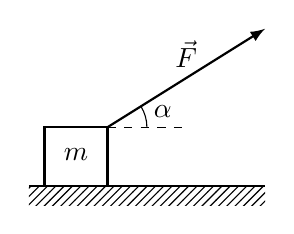
\begin{tikzpicture}
	\coordinate (A) at (2, 0.75);
    \coordinate (B) at (1, 0.75);
    \coordinate (C) at (3, 2);
       
	\draw [draw=none, pattern=north east lines] (0,-0.25) rectangle (3, 0);	
	\draw [thick] (0, 0) -- (3, 0);

	\draw [thick] (B) rectangle (0.2, 0);
	\draw [dashed] (B) -- (A);
	\node at (0.6, 0.4) {$m$};
	
	\draw [arrows={-latex}, thick] (B) -- (C) node [above, midway]  {$\vec{F}$};
	
	\pic [draw, -, angle eccentricity=1.5] {angle = A--B--C};
	\node [right=20pt, above] at (B) {$\alpha$};
\end{tikzpicture}
\end{document}